%%%%%%%%%%%%%%%%%%%%%%%%%%%%%%%%%%%%%%%%%
% Journal Article
% LaTeX Template
% Version 1.3 (9/9/13)
%
% This template has been downloaded from:
% http://www.LaTeXTemplates.com
%
% Original author:
% Frits Wenneker (http://www.howtotex.com)
%
% License:
% CC BY-NC-SA 3.0 (http://creativecommons.org/licenses/by-nc-sa/3.0/)
%
%%%%%%%%%%%%%%%%%%%%%%%%%%%%%%%%%%%%%%%%%

%----------------------------------------------------------------------------------------
%	PACKAGES AND OTHER DOCUMENT CONFIGURATIONS
%----------------------------------------------------------------------------------------

\documentclass[twoside]{article}


\usepackage[utf8]{inputenc} % Permite el uso de acentos directamente
\usepackage[sc]{mathpazo} % Use the Palatino font
\usepackage[T1]{fontenc} % Use 8-bit encoding that has 256 glyphs
\linespread{1.05} % Line spacing - Palatino needs more space between lines
\usepackage{microtype} % Slightly tweak font spacing for aesthetics
\usepackage{adjustbox}
\usepackage{amsmath} % Equations
\usepackage{amssymb} % Equations
\usepackage{color} % Allow colors to be defined
\usepackage{enumerate} % Needed for markdown enumerations to work
\usepackage{fancyvrb} % verbatim replacement that allows latex
\usepackage[hmarginratio=1:1,top=32mm,columnsep=20pt]{geometry} % Document margins
\usepackage{multicol} % Used for the two-column layout of the document
\usepackage[hang, small,labelfont=bf,up,textfont=it,up]{caption} % Custom captions under/above floats in tables or figures
\usepackage{booktabs} % Horizontal rules in tables
\usepackage{float} % Required for tables and figures in the multi-column environment - they need to be placed in specific locations with the [H] (e.g. \begin{table}[H])
\usepackage{hyperref} % For hyperlinks in the PDF
\usepackage{multirow} % para las tablas
\usepackage{lettrine} % The lettrine is the first enlarged letter at the beginning of the text
\usepackage{paralist} % Used for the compactitem environment which makes bullet points with less space between them

\usepackage{abstract} % Allows abstract customization
\renewcommand{\abstractnamefont}{\normalfont\bfseries} % Set the "Abstract" text to bold
\renewcommand{\abstracttextfont}{\normalfont\small\itshape} % Set the abstract itself to small italic text

\usepackage{titlesec} % Allows customization of titles
\renewcommand\thesection{\Roman{section}} % Roman numerals for the sections
\renewcommand\thesubsection{\Roman{subsection}} % Roman numerals for subsections
\titleformat{\section}[block]{\large\scshape\centering}{\thesection.}{1em}{} % Change the look of the section titles
\titleformat{\subsection}[block]{\large}{\thesubsection.}{1em}{} % Change the look of the section titles

\usepackage{fancyhdr} % Headers and footers
\pagestyle{fancy} % All pages have headers and footers
\fancyhead{} % Blank out the default header
\fancyfoot{} % Blank out the default footer
\fancyhead[C]{ESTUDIO DE LA CINEMÁTICA DIRECTA Y CINEMÁTICA INVERSA DE UN MANIPULADOR PLANO DE 3 GRADOS DE LIBERTAD  $\bullet$ Junio 2015 $\bullet$} % Custom header text
\fancyfoot[RO,LE]{\thepage} % Custom footer text
\usepackage{graphicx}
\definecolor{orange}{cmyk}{0,0.4,0.8,0.2}
    \definecolor{darkorange}{rgb}{.71,0.21,0.01}
    \definecolor{darkgreen}{rgb}{.12,.54,.11}
    \definecolor{myteal}{rgb}{.26, .44, .56}
    \definecolor{gray}{gray}{0.45}
    \definecolor{lightgray}{gray}{.95}
    \definecolor{mediumgray}{gray}{.8}
    \definecolor{inputbackground}{rgb}{.95, .95, .85}
    \definecolor{outputbackground}{rgb}{.95, .95, .95}
    \definecolor{traceback}{rgb}{1, .95, .95}
    % ansi colors
    \definecolor{red}{rgb}{.6,0,0}
    \definecolor{green}{rgb}{0,.65,0}
    \definecolor{brown}{rgb}{0.6,0.6,0}
    \definecolor{blue}{rgb}{0,.145,.698}
    \definecolor{purple}{rgb}{.698,.145,.698}
    \definecolor{cyan}{rgb}{0,.698,.698}
    \definecolor{lightgray}{gray}{0.5}
    
    % bright ansi colors
    \definecolor{darkgray}{gray}{0.25}
    \definecolor{lightred}{rgb}{1.0,0.39,0.28}
    \definecolor{lightgreen}{rgb}{0.48,0.99,0.0}
    \definecolor{lightblue}{rgb}{0.53,0.81,0.92}
    \definecolor{lightpurple}{rgb}{0.87,0.63,0.87}
    \definecolor{lightcyan}{rgb}{0.5,1.0,0.83}
    
    % commands and environments needed by pandoc snippets
    % extracted from the output of `pandoc -s`
    \providecommand{\tightlist}{%
      \setlength{\itemsep}{0pt}\setlength{\parskip}{0pt}}
    \DefineVerbatimEnvironment{Highlighting}{Verbatim}{commandchars=\\\{\}}
    % Add ',fontsize=\small' for more characters per line
    \newenvironment{Shaded}{}{}
    \newcommand{\KeywordTok}[1]{\textcolor[rgb]{0.00,0.44,0.13}{\textbf{{#1}}}}
    \newcommand{\DataTypeTok}[1]{\textcolor[rgb]{0.56,0.13,0.00}{{#1}}}
    \newcommand{\DecValTok}[1]{\textcolor[rgb]{0.25,0.63,0.44}{{#1}}}
    \newcommand{\BaseNTok}[1]{\textcolor[rgb]{0.25,0.63,0.44}{{#1}}}
    \newcommand{\FloatTok}[1]{\textcolor[rgb]{0.25,0.63,0.44}{{#1}}}
    \newcommand{\CharTok}[1]{\textcolor[rgb]{0.25,0.44,0.63}{{#1}}}
    \newcommand{\StringTok}[1]{\textcolor[rgb]{0.25,0.44,0.63}{{#1}}}
    \newcommand{\CommentTok}[1]{\textcolor[rgb]{0.38,0.63,0.69}{\textit{{#1}}}}
    \newcommand{\OtherTok}[1]{\textcolor[rgb]{0.00,0.44,0.13}{{#1}}}
    \newcommand{\AlertTok}[1]{\textcolor[rgb]{1.00,0.00,0.00}{\textbf{{#1}}}}
    \newcommand{\FunctionTok}[1]{\textcolor[rgb]{0.02,0.16,0.49}{{#1}}}
    \newcommand{\RegionMarkerTok}[1]{{#1}}
    \newcommand{\ErrorTok}[1]{\textcolor[rgb]{1.00,0.00,0.00}{\textbf{{#1}}}}
    \newcommand{\NormalTok}[1]{{#1}}
    
    % Define a nice break command that doesn't care if a line doesn't already
    % exist.
    \def\br{\hspace*{\fill} \\* }
    % Math Jax compatability definitions
    \def\gt{>}
    \def\lt{<}
    % Document parameters
    \title{C?digo\_Proyecto\_2\_de\_robotica}
    
    
    

    % Pygments definitions
    
\makeatletter
\def\PY@reset{\let\PY@it=\relax \let\PY@bf=\relax%
    \let\PY@ul=\relax \let\PY@tc=\relax%
    \let\PY@bc=\relax \let\PY@ff=\relax}
\def\PY@tok#1{\csname PY@tok@#1\endcsname}
\def\PY@toks#1+{\ifx\relax#1\empty\else%
    \PY@tok{#1}\expandafter\PY@toks\fi}
\def\PY@do#1{\PY@bc{\PY@tc{\PY@ul{%
    \PY@it{\PY@bf{\PY@ff{#1}}}}}}}
\def\PY#1#2{\PY@reset\PY@toks#1+\relax+\PY@do{#2}}

\expandafter\def\csname PY@tok@gd\endcsname{\def\PY@tc##1{\textcolor[rgb]{0.63,0.00,0.00}{##1}}}
\expandafter\def\csname PY@tok@gu\endcsname{\let\PY@bf=\textbf\def\PY@tc##1{\textcolor[rgb]{0.50,0.00,0.50}{##1}}}
\expandafter\def\csname PY@tok@gt\endcsname{\def\PY@tc##1{\textcolor[rgb]{0.00,0.27,0.87}{##1}}}
\expandafter\def\csname PY@tok@gs\endcsname{\let\PY@bf=\textbf}
\expandafter\def\csname PY@tok@gr\endcsname{\def\PY@tc##1{\textcolor[rgb]{1.00,0.00,0.00}{##1}}}
\expandafter\def\csname PY@tok@cm\endcsname{\let\PY@it=\textit\def\PY@tc##1{\textcolor[rgb]{0.25,0.50,0.50}{##1}}}
\expandafter\def\csname PY@tok@vg\endcsname{\def\PY@tc##1{\textcolor[rgb]{0.10,0.09,0.49}{##1}}}
\expandafter\def\csname PY@tok@m\endcsname{\def\PY@tc##1{\textcolor[rgb]{0.40,0.40,0.40}{##1}}}
\expandafter\def\csname PY@tok@mh\endcsname{\def\PY@tc##1{\textcolor[rgb]{0.40,0.40,0.40}{##1}}}
\expandafter\def\csname PY@tok@go\endcsname{\def\PY@tc##1{\textcolor[rgb]{0.53,0.53,0.53}{##1}}}
\expandafter\def\csname PY@tok@ge\endcsname{\let\PY@it=\textit}
\expandafter\def\csname PY@tok@vc\endcsname{\def\PY@tc##1{\textcolor[rgb]{0.10,0.09,0.49}{##1}}}
\expandafter\def\csname PY@tok@il\endcsname{\def\PY@tc##1{\textcolor[rgb]{0.40,0.40,0.40}{##1}}}
\expandafter\def\csname PY@tok@cs\endcsname{\let\PY@it=\textit\def\PY@tc##1{\textcolor[rgb]{0.25,0.50,0.50}{##1}}}
\expandafter\def\csname PY@tok@cp\endcsname{\def\PY@tc##1{\textcolor[rgb]{0.74,0.48,0.00}{##1}}}
\expandafter\def\csname PY@tok@gi\endcsname{\def\PY@tc##1{\textcolor[rgb]{0.00,0.63,0.00}{##1}}}
\expandafter\def\csname PY@tok@gh\endcsname{\let\PY@bf=\textbf\def\PY@tc##1{\textcolor[rgb]{0.00,0.00,0.50}{##1}}}
\expandafter\def\csname PY@tok@ni\endcsname{\let\PY@bf=\textbf\def\PY@tc##1{\textcolor[rgb]{0.60,0.60,0.60}{##1}}}
\expandafter\def\csname PY@tok@nl\endcsname{\def\PY@tc##1{\textcolor[rgb]{0.63,0.63,0.00}{##1}}}
\expandafter\def\csname PY@tok@nn\endcsname{\let\PY@bf=\textbf\def\PY@tc##1{\textcolor[rgb]{0.00,0.00,1.00}{##1}}}
\expandafter\def\csname PY@tok@no\endcsname{\def\PY@tc##1{\textcolor[rgb]{0.53,0.00,0.00}{##1}}}
\expandafter\def\csname PY@tok@na\endcsname{\def\PY@tc##1{\textcolor[rgb]{0.49,0.56,0.16}{##1}}}
\expandafter\def\csname PY@tok@nb\endcsname{\def\PY@tc##1{\textcolor[rgb]{0.00,0.50,0.00}{##1}}}
\expandafter\def\csname PY@tok@nc\endcsname{\let\PY@bf=\textbf\def\PY@tc##1{\textcolor[rgb]{0.00,0.00,1.00}{##1}}}
\expandafter\def\csname PY@tok@nd\endcsname{\def\PY@tc##1{\textcolor[rgb]{0.67,0.13,1.00}{##1}}}
\expandafter\def\csname PY@tok@ne\endcsname{\let\PY@bf=\textbf\def\PY@tc##1{\textcolor[rgb]{0.82,0.25,0.23}{##1}}}
\expandafter\def\csname PY@tok@nf\endcsname{\def\PY@tc##1{\textcolor[rgb]{0.00,0.00,1.00}{##1}}}
\expandafter\def\csname PY@tok@si\endcsname{\let\PY@bf=\textbf\def\PY@tc##1{\textcolor[rgb]{0.73,0.40,0.53}{##1}}}
\expandafter\def\csname PY@tok@s2\endcsname{\def\PY@tc##1{\textcolor[rgb]{0.73,0.13,0.13}{##1}}}
\expandafter\def\csname PY@tok@vi\endcsname{\def\PY@tc##1{\textcolor[rgb]{0.10,0.09,0.49}{##1}}}
\expandafter\def\csname PY@tok@nt\endcsname{\let\PY@bf=\textbf\def\PY@tc##1{\textcolor[rgb]{0.00,0.50,0.00}{##1}}}
\expandafter\def\csname PY@tok@nv\endcsname{\def\PY@tc##1{\textcolor[rgb]{0.10,0.09,0.49}{##1}}}
\expandafter\def\csname PY@tok@s1\endcsname{\def\PY@tc##1{\textcolor[rgb]{0.73,0.13,0.13}{##1}}}
\expandafter\def\csname PY@tok@kd\endcsname{\let\PY@bf=\textbf\def\PY@tc##1{\textcolor[rgb]{0.00,0.50,0.00}{##1}}}
\expandafter\def\csname PY@tok@sh\endcsname{\def\PY@tc##1{\textcolor[rgb]{0.73,0.13,0.13}{##1}}}
\expandafter\def\csname PY@tok@sc\endcsname{\def\PY@tc##1{\textcolor[rgb]{0.73,0.13,0.13}{##1}}}
\expandafter\def\csname PY@tok@sx\endcsname{\def\PY@tc##1{\textcolor[rgb]{0.00,0.50,0.00}{##1}}}
\expandafter\def\csname PY@tok@bp\endcsname{\def\PY@tc##1{\textcolor[rgb]{0.00,0.50,0.00}{##1}}}
\expandafter\def\csname PY@tok@c1\endcsname{\let\PY@it=\textit\def\PY@tc##1{\textcolor[rgb]{0.25,0.50,0.50}{##1}}}
\expandafter\def\csname PY@tok@kc\endcsname{\let\PY@bf=\textbf\def\PY@tc##1{\textcolor[rgb]{0.00,0.50,0.00}{##1}}}
\expandafter\def\csname PY@tok@c\endcsname{\let\PY@it=\textit\def\PY@tc##1{\textcolor[rgb]{0.25,0.50,0.50}{##1}}}
\expandafter\def\csname PY@tok@mf\endcsname{\def\PY@tc##1{\textcolor[rgb]{0.40,0.40,0.40}{##1}}}
\expandafter\def\csname PY@tok@err\endcsname{\def\PY@bc##1{\setlength{\fboxsep}{0pt}\fcolorbox[rgb]{1.00,0.00,0.00}{1,1,1}{\strut ##1}}}
\expandafter\def\csname PY@tok@mb\endcsname{\def\PY@tc##1{\textcolor[rgb]{0.40,0.40,0.40}{##1}}}
\expandafter\def\csname PY@tok@ss\endcsname{\def\PY@tc##1{\textcolor[rgb]{0.10,0.09,0.49}{##1}}}
\expandafter\def\csname PY@tok@sr\endcsname{\def\PY@tc##1{\textcolor[rgb]{0.73,0.40,0.53}{##1}}}
\expandafter\def\csname PY@tok@mo\endcsname{\def\PY@tc##1{\textcolor[rgb]{0.40,0.40,0.40}{##1}}}
\expandafter\def\csname PY@tok@kn\endcsname{\let\PY@bf=\textbf\def\PY@tc##1{\textcolor[rgb]{0.00,0.50,0.00}{##1}}}
\expandafter\def\csname PY@tok@mi\endcsname{\def\PY@tc##1{\textcolor[rgb]{0.40,0.40,0.40}{##1}}}
\expandafter\def\csname PY@tok@gp\endcsname{\let\PY@bf=\textbf\def\PY@tc##1{\textcolor[rgb]{0.00,0.00,0.50}{##1}}}
\expandafter\def\csname PY@tok@o\endcsname{\def\PY@tc##1{\textcolor[rgb]{0.40,0.40,0.40}{##1}}}
\expandafter\def\csname PY@tok@kr\endcsname{\let\PY@bf=\textbf\def\PY@tc##1{\textcolor[rgb]{0.00,0.50,0.00}{##1}}}
\expandafter\def\csname PY@tok@s\endcsname{\def\PY@tc##1{\textcolor[rgb]{0.73,0.13,0.13}{##1}}}
\expandafter\def\csname PY@tok@kp\endcsname{\def\PY@tc##1{\textcolor[rgb]{0.00,0.50,0.00}{##1}}}
\expandafter\def\csname PY@tok@w\endcsname{\def\PY@tc##1{\textcolor[rgb]{0.73,0.73,0.73}{##1}}}
\expandafter\def\csname PY@tok@kt\endcsname{\def\PY@tc##1{\textcolor[rgb]{0.69,0.00,0.25}{##1}}}
\expandafter\def\csname PY@tok@ow\endcsname{\let\PY@bf=\textbf\def\PY@tc##1{\textcolor[rgb]{0.67,0.13,1.00}{##1}}}
\expandafter\def\csname PY@tok@sb\endcsname{\def\PY@tc##1{\textcolor[rgb]{0.73,0.13,0.13}{##1}}}
\expandafter\def\csname PY@tok@k\endcsname{\let\PY@bf=\textbf\def\PY@tc##1{\textcolor[rgb]{0.00,0.50,0.00}{##1}}}
\expandafter\def\csname PY@tok@se\endcsname{\let\PY@bf=\textbf\def\PY@tc##1{\textcolor[rgb]{0.73,0.40,0.13}{##1}}}
\expandafter\def\csname PY@tok@sd\endcsname{\let\PY@it=\textit\def\PY@tc##1{\textcolor[rgb]{0.73,0.13,0.13}{##1}}}

\def\PYZbs{\char`\\}
\def\PYZus{\char`\_}
\def\PYZob{\char`\{}
\def\PYZcb{\char`\}}
\def\PYZca{\char`\^}
\def\PYZam{\char`\&}
\def\PYZlt{\char`\<}
\def\PYZgt{\char`\>}
\def\PYZsh{\char`\#}
\def\PYZpc{\char`\%}
\def\PYZdl{\char`\$}
\def\PYZhy{\char`\-}
\def\PYZsq{\char`\'}
\def\PYZdq{\char`\"}
\def\PYZti{\char`\~}
% for compatibility with earlier versions
\def\PYZat{@}
\def\PYZlb{[}
\def\PYZrb{]}
\makeatother


    % Exact colors from NB
    \definecolor{incolor}{rgb}{0.0, 0.0, 0.5}
    \definecolor{outcolor}{rgb}{0.545, 0.0, 0.0}



    
    % Prevent overflowing lines due to hard-to-break entities
    \sloppy 
    % Setup hyperref package
    \hypersetup{
      breaklinks=true,  % so long urls are correctly broken across lines
      colorlinks=true,
      urlcolor=blue,
      linkcolor=darkorange,
      citecolor=darkgreen,
      }
    % Slightly bigger margins than the latex defaults
    
    \geometry{verbose,tmargin=1in,bmargin=1in,lmargin=1in,rmargin=1in}
    

%----------------------------------------------------------------------------------------
%	TITLE SECTION
%----------------------------------------------------------------------------------------

\title{\vspace{-15mm}\fontsize{24pt}{10pt}\selectfont\textbf{ESTUDIO DE LA CINEMÁTICA DIRECTA Y CINEMÁTICA INVERSA DE UN MANIPULADOR PLANO DE 3 GRADOS DE LIBERTAD}} % Article title

\author{
\large
\textsc{Eduardo Vieira}\\% Your name 
\normalsize Universidad Central de Venezuela \\ % Your institution
\normalsize Facultad de Ingeniería \\
\normalsize Escuela de Ingeniería Mecánica \\
\normalsize eduardo.vieira@ucv.ve \\ % Your email address
\normalsize Profesor: Arturo Gil \\
\vspace{-5mm}
}
\date{}

%----------------------------------------------------------------------------------------

\begin{document}

\maketitle % Insert title

\thispagestyle{fancy} % All pages have headers and footers

%----------------------------------------------------------------------------------------
%	ABSTRACT
%----------------------------------------------------------------------------------------

%\begin{abstract}

%\noindent \lipsum[1] % Dummy abstract text

%\end{abstract}

%----------------------------------------------------------------------------------------
%	ARTICLE CONTENTS
%----------------------------------------------------------------------------------------

\begin{multicols}{2} % Two-column layout throughout the main article text

\section{Introducción}

\lettrine[nindent=0em,lines=3]{L} a cinemática del robot estudia el movimiento del mismo con respecto a un sistema de referencia sin considerar las fuerzas que intervienen. Así, la cinemática se interesa por la descripción analítica del movimiento espacial del robot como una función del tiempo, y en particular por las relaciones entre la posición y la orientación del extremo final del robot con los valores que toman sus coordenadas articulares. \\
Existen dos problemas fundamentales a resolver en la cinemática del robot, el primero de ellos se conoce como el problema cinemático directo, y consiste en determinar cuál es la posición y orientación del extremo final del robot, con respecto a un sistema de coordenadas que se toma como referencia, conocidos los valores de las articulaciones y los parámetros geométricos de los elementos del robot; el segundo, denominado problema cinemático inverso, resuelve la configuración que debe adoptar el robot para una posición y orientación en su extremo conocidas. \\
En el presente trabajo se estudiará el problema cinemático directo e inverso para un manipulador plano de 3 grados de libertad.  Además de desarrollará un algoritmo en python para la solución interactiva del problema.

%------------------------------------------------

\section{El Problema}
\subsection{Se tiene}
\textbf{Se tiene:} El siguiente manipulador plano \\
\begin{center}
 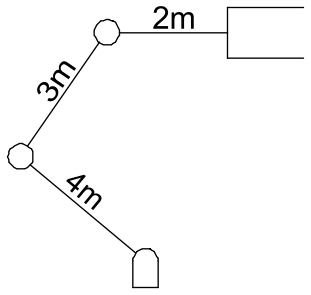
\includegraphics[width=200pt,keepaspectratio=true]{./Robot.png}
 % P&ID_anti-suge.png: 0x0 pixel, 300dpi, 0.00x0.00 cm, bb=
  \textit{Figura 1: Manipulador plano de 3 grados de libertad}
\end{center}


\subsection{Se pide}
\begin{enumerate}
\def\labelenumi{\arabic{enumi}.}
\itemsep1pt\parskip0pt\parsep0pt
\item
  Definir la matriz de Denvit-Hatenberg.

\def\labelenumii{\arabic{enumii}.}
\setcounter{enumii}{1}
\itemsep1pt\parskip0pt\parsep0pt
\item
  Estudiar la cinématica directa.

\def\labelenumiii{\arabic{enumiii}.}
\setcounter{enumiii}{2}
\itemsep1pt\parskip0pt\parsep0pt
\item
   Estudiar la cinématica inversa.

\end{enumerate}


\subsection{Cinemática Directa}
\subsubsection{Algoritmo de Denavit-Hartenberg}
\begin{enumerate}
\def\labelenumi{\arabic{enumi}.}
\itemsep1pt\parskip0pt\parsep0pt
\item
  Numerar los eslabones comenzando con \(1\) (primer eslabón móvil dela
  cadena) y acabando con \(n\) (último eslabón móvil). Se numerará como
  eslabón \(0\) a la base fija del robot.
\end{enumerate}

\begin{enumerate}
\def\labelenumi{\arabic{enumi}.}
\setcounter{enumi}{1}
\itemsep1pt\parskip0pt\parsep0pt
\item
  Numerar cada articulación comenzando por \(1\) (la correspondiente al
  primer grado de libertad) y acabando en \(n\).
\end{enumerate}

\begin{enumerate}
\def\labelenumi{\arabic{enumi}.}
\setcounter{enumi}{2}
\itemsep1pt\parskip0pt\parsep0pt
\item
  Localizar el eje de cada articulación. Si esta es rotativa, el eje
  será su propio eje de giro. Si es prismática, será el eje a lo largo
  del cual se produce el desplazamiento.
\end{enumerate}

\begin{enumerate}
\def\labelenumi{\arabic{enumi}.}
\setcounter{enumi}{3}
\itemsep1pt\parskip0pt\parsep0pt
\item
  Para \(i\) de \(0\) a \(n-1\), situar el eje \(Z_i\), sobre el eje de
  la articulación \(i+1\).
\end{enumerate}

\begin{enumerate}
\def\labelenumi{\arabic{enumi}.}
\setcounter{enumi}{4}
\itemsep1pt\parskip0pt\parsep0pt
\item
  Situar el origen del sistema de la base (\(S_0\)) en cualquier punto
  del eje \(Z_0\). Los ejes \(X_0\) e \(Y_0\) se situaran dé modo que
  formen un sistema dextrógiro con \(Z_0\).
\end{enumerate}

\begin{enumerate}
\def\labelenumi{\arabic{enumi}.}
\setcounter{enumi}{5}
\itemsep1pt\parskip0pt\parsep0pt
\item
  Para \(i\) de \(1\) a \(n-1\), situar el sistema (\(S_i\)) (solidario
  al eslabón \(i\)) en la intersección del eje \(Z_i\) con la línea
  normal común a \(Z_{i-1}\) y \(Z_i\). Si ambos ejes se cortasen se
  situaría (\(S_i\)) en el punto de corte. Si fuesen paralelos (\(S_i\))
  se situaría en la articulación \(i+1\).
\end{enumerate}

\begin{enumerate}
\def\labelenumi{\arabic{enumi}.}
\setcounter{enumi}{6}
\itemsep1pt\parskip0pt\parsep0pt
\item
  Situar $X_i$ en la línea normal común a $Z_{i-1}$ y $Z_{i}$.
\end{enumerate}

\begin{enumerate}
\def\labelenumi{\arabic{enumi}.}
\setcounter{enumi}{7}
\itemsep1pt\parskip0pt\parsep0pt
\item
  Situar $Y_i$ de modo que forme un sistema dextrógiro con $X_i$ y $Z_i$.
\end{enumerate}

\begin{enumerate}
\def\labelenumi{\arabic{enumi}.}
\setcounter{enumi}{8}
\itemsep1pt\parskip0pt\parsep0pt
\item
  Situar el sistema ($S_n$) en el extremo del robot de modo que $Z_n$ coincida
  con la dirección de $Z_{n-1}$ y $X_n$ sea normal a $Z_{n-1}$ y $Z_n$.
\end{enumerate}

\begin{enumerate}
\def\labelenumi{\arabic{enumi}.}
\setcounter{enumi}{9}
\itemsep1pt\parskip0pt\parsep0pt
\item
  Obtener $\theta_i$ como el ángulo que hay que girar en torno a $Z_{i-1}$ para que
  $X_{i-1}$ y $X_i$ queden paralelos.
\end{enumerate}

\begin{enumerate}
\def\labelenumi{\arabic{enumi}.}
\setcounter{enumi}{10}
\itemsep1pt\parskip0pt\parsep0pt
\item
  Obtener $D_i$ como la distancia, medida a lo largo de $Z_{i-1}$, que habría
  que desplazar ($S_{i-1}$) para que $X_i$ y $X_{i-1}$ quedasen alineados.
\end{enumerate}

\begin{enumerate}
\def\labelenumi{\arabic{enumi}.}
\setcounter{enumi}{11}
\itemsep1pt\parskip0pt\parsep0pt
\item
  Obtener $A_i$ como la distancia medida a lo largo de $X_i$ (que ahora
  coincidiría con $X_{i-1}$) que habría que desplazar el nuevo ($S_{i-1}$) para
  que su origen coincidiese con ($S_i$).
\end{enumerate}

\begin{enumerate}
\def\labelenumi{\arabic{enumi}.}
\setcounter{enumi}{12}
\itemsep1pt\parskip0pt\parsep0pt
\item
  Obtener $\alpha_i$ como el ángulo que habría que girar entorno a $X_i$ (que ahora
  coincidiría con $X_{i-1}$), para que el nuevo ($S_{i-1}$) coincidiese totalmente
  con ($S_i$).
\end{enumerate}

\begin{enumerate}
\def\labelenumi{\arabic{enumi}.}
\setcounter{enumi}{13}
\itemsep1pt\parskip0pt\parsep0pt
\item
  Obtener las matrices de transformación $^{i-1}A_i$.
\end{enumerate}

\begin{enumerate}
\def\labelenumi{\arabic{enumi}.}
\setcounter{enumi}{14}
\itemsep1pt\parskip0pt\parsep0pt
\item
  Obtener la matriz de transformación que relaciona el sistema de la
  base con el del extremo del robot $T = ^0A_i  ^1A_2\ldots{} ^{n-1}A_n$.
\end{enumerate}

\begin{enumerate}
\def\labelenumi{\arabic{enumi}.}
\setcounter{enumi}{15}
\itemsep1pt\parskip0pt\parsep0pt
\item
  La matriz $T$ define la orientación (submatriz de rotación) y posición
  (submatriz de traslación) del extremo referido ala base en función de
  las n coordenadas articulares.
\end{enumerate}

Al aplicar el algorítmo quedaría
\begin{center}
 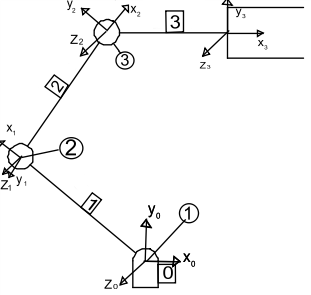
\includegraphics[width=200pt,keepaspectratio=true]{./RobotDH5.png}
 % P&ID_anti-suge.png: 0x0 pixel, 300dpi, 0.00x0.00 cm, bb=
  \textit{Figura 2: Algoritmo de Denavit-Hartenberg aplicado al manipulador}
\end{center}
Los paŕametros para cada articulación son

\begin{center}
 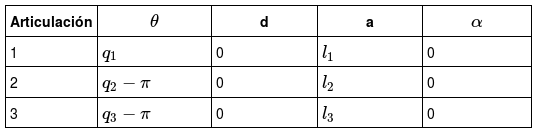
\includegraphics[width=240pt,keepaspectratio=true]{./Tabla_DH.png}
 % P&ID_anti-suge.png: 0x0 pixel, 300dpi, 0.00x0.00 cm, bb=
  \textit{Tabla 1: Parámetros de Denavit-Hartenberg}
\end{center}

La matriz de transformación \(^{0}T_{1}\) será
\begin{equation}
 \left[\begin{matrix}\cos{\left (q_{1} \right )} & - \sin{\left (q_{1} \right )} & 0 & 4 \cos{\left (q_{1} \right )}\\\sin{\left (q_{1} \right )} & \cos{\left (q_{1} \right )} & 0 & 4 \sin{\left (q_{1} \right )}\\0 & 0 & 1 & 0\\0 & 0 & 0 & 1\end{matrix}\right]
\end{equation} 

$^{1}T_{2}$
\begin{equation}
 \left[\begin{matrix}- \cos{\left (q_{2} \right )} & \sin{\left (q_{2} \right )} & 0 & - 3 \cos{\left (q_{2} \right )}\\- \sin{\left (q_{2} \right )} & - \cos{\left (q_{2} \right )} & 0 & - 3 \sin{\left (q_{2} \right )}\\0 & 0 & 1 & 0\\0 & 0 & 0 & 1\end{matrix}\right]
\end{equation}

Y finalmente $^{2}T_{3}$
\begin{equation}
 \left[\begin{matrix}- \cos{\left (q_{3} \right )} & \sin{\left (q_{3} \right )} & 0 & - 2 \cos{\left (q_{3} \right )}\\- \sin{\left (q_{3} \right )} & - \cos{\left (q_{3} \right )} & 0 & - 2 \sin{\left (q_{3} \right )}\\0 & 0 & 1 & 0\\0 & 0 & 0 & 1\end{matrix}\right]
\end{equation} 

La matriz de transformación que relaciona el extremo de la herramienta del robot con el sistema definido en la base $T$ será $T = ^{0}T_{1} \cdot ^{1}T_{2} \cdot ^{2}T_{3}$

\begin{equation}
\left[\begin{matrix}\alpha & \beta & 0 & \gamma\\\ \delta & \epsilon & 0 & \kappa \\0 & 0 & 1 & 0\\0 & 0 & 0 & 1\end{matrix}\right]
\end{equation} 
Donde $\alpha=- \left(\sin{\left (q_{1} \right )} \sin{\left (q_{2} \right )} - \cos{\left (q_{1} \right )} \cos{\left (q_{2} \right )}\right) \cos{\left (q_{3} \right )} - \left(\sin{\left (q_{1} \right )} \cos{\left (q_{2} \right )} + \sin{\left (q_{2} \right )} \cos{\left (q_{1} \right )}\right) \sin{\left (q_{3} \right )}$ \\

\vspace*{1\baselineskip}
$\beta=\left(\sin{\left (q_{1} \right )} \sin{\left (q_{2} \right )} - \cos{\left (q_{1} \right )} \cos{\left (q_{2} \right )}\right) \sin{\left (q_{3} \right )} - \left(\sin{\left (q_{1} \right )} \cos{\left (q_{2} \right )} + \sin{\left (q_{2} \right )} \cos{\left (q_{1} \right )}\right) \cos{\left (q_{3} \right )}$ \\

\vspace*{1\baselineskip}
$\gamma=- 2 \left(\sin{\left (q_{1} \right )} \sin{\left (q_{2} \right )} - \cos{\left (q_{1} \right )} \cos{\left (q_{2} \right )}\right) \cos{\left (q_{3} \right )} - 2 \left(\sin{\left (q_{1} \right )} \cos{\left (q_{2} \right )} + \sin{\left (q_{2} \right )} \cos{\left (q_{1} \right )}\right) \sin{\left (q_{3} \right )} + 3 \sin{\left (q_{1} \right )} \sin{\left (q_{2} \right )} - 3 \cos{\left (q_{1} \right )} \cos{\left (q_{2} \right )} + 4 \cos{\left (q_{1} \right )}$\\

\vspace*{1\baselineskip}
$\delta=- \left(\sin{\left (q_{1} \right )} \sin{\left (q_{2} \right )} - \cos{\left (q_{1} \right )} \cos{\left (q_{2} \right )}\right) \sin{\left (q_{3} \right )} - \left(- \sin{\left (q_{1} \right )} \cos{\left (q_{2} \right )} - \sin{\left (q_{2} \right )} \cos{\left (q_{1} \right )}\right) \cos{\left (q_{3} \right )} $\\

\vspace*{1\baselineskip}
$\epsilon=- \left(\sin{\left (q_{1} \right )} \sin{\left (q_{2} \right )} - \cos{\left (q_{1} \right )} \cos{\left (q_{2} \right )}\right) \cos{\left (q_{3} \right )} + \left(- \sin{\left (q_{1} \right )} \cos{\left (q_{2} \right )} - \sin{\left (q_{2} \right )} \cos{\left (q_{1} \right )}\right) \sin{\left (q_{3} \right )} $\\

\vspace*{1\baselineskip}
$\kappa=- 2 \left(\sin{\left (q_{1} \right )} \sin{\left (q_{2} \right )} - \cos{\left (q_{1} \right )} \cos{\left (q_{2} \right )}\right) \sin{\left (q_{3} \right )} - 2 \left(- \sin{\left (q_{1} \right )} \cos{\left (q_{2} \right )} - \sin{\left (q_{2} \right )} \cos{\left (q_{1} \right )}\right) \cos{\left (q_{3} \right )} - 3 \sin{\left (q_{1} \right )} \cos{\left (q_{2} \right )} + 4 \sin{\left (q_{1} \right )} - 3 \sin{\left (q_{2} \right )} \cos{\left (q_{1} \right )}$
\vspace*{1\baselineskip}
Sean $x_r$, $y_r$ y $z_r$ las coordenadas de un punto medidas desde el sistema de referencia ubicado en el extremo del robot.
\begin{equation}
 P_r = \left[\begin{matrix}x_{r}\\y_{r}\\z_{r}\\1\end{matrix}\right]
\end{equation} 
Entonces, el mismo punto medido en el sistema de referencia de la base será $T \cdot P_r$

 
$x = x_{r} (- (\sin{ (q_{1}  )} \sin{ (q_{2}  )} - \cos{ (q_{1}  )} \cos{ (q_{2}  )}) \cos{ (q_{3}  )} \\ - (\sin{ (q_{1}  )} \cos{ (q_{2}  )} + \sin{ (q_{2}  )} \cos{ (q_{1}  )}) \sin{ (q_{3}  )}) + y_{r} ((\sin{ (q_{1}  )} \sin{ (q_{2}  )} - \cos{ (q_{1}  )} \cos{ (q_{2}  )}) \sin{ (q_{3}  )} - (\sin{ (q_{1}  )} \cos{ (q_{2}  )} + \sin{ (q_{2}  )} \cos{ (q_{1}  )}) \cos{ (q_{3}  )}) - 2 (\sin{ (q_{1}  )} \sin{ (q_{2}  )} - \cos{ (q_{1}  )} \cos{ (q_{2}  )}) \cos{ (q_{3}  )} - 2 (\sin{ (q_{1}  )} \cos{ (q_{2}  )} + \sin{ (q_{2}  )} \cos{ (q_{1}  )}) \sin{ (q_{3}  )} + 3 \sin{ (q_{1}  )} \sin{ (q_{2}  )} - 3 \cos{ (q_{1}  )} \cos{ (q_{2}  )} + 4 \cos{ (q_{1}  )}$\\

\vspace*{1\baselineskip}
$y = x_{r} (- (\sin{ (q_{1}  )} \sin{ (q_{2}  )} - \cos{ (q_{1}  )} \cos{ (q_{2}  )}) \sin{ (q_{3}  )} - (- \sin{ (q_{1}  )} \cos{ (q_{2}  )} - \sin{ (q_{2}  )} \cos{ (q_{1}  )}) \cos{ (q_{3}  )}) + y_{r} (- (\sin{ (q_{1}  )} \sin{ (q_{2}  )} - \cos{ (q_{1}  )} \cos{ (q_{2}  )}) \cos{ (q_{3}  )} + (- \sin{ (q_{1}  )} \cos{ (q_{2}  )} - \sin{ (q_{2}  )} \cos{ (q_{1}  )}) \sin{ (q_{3}  )}) - 2 (\sin{ (q_{1}  )} \sin{ (q_{2}  )} - \cos{ (q_{1}  )} \cos{ (q_{2}  )}) \sin{ (q_{3}  )} - 2 (- \sin{ (q_{1}  )} \cos{ (q_{2}  )} - \sin{ (q_{2}  )} \cos{ (q_{1}  )}) \cos{ (q_{3}  )} - 3 \sin{ (q_{1}  )} \cos{ (q_{2}  )} + 4 \sin{ (q_{1}  )} - 3 \sin{ (q_{2}  )} \cos{ (q_{1}  )}$
\vspace*{1\baselineskip}

Si colocamos el sistema de referencia en la base ($x_r$ y $y_r$ iguales a cero) el punto que determina la ubicación de la
herramienta se obtiene de la siguiente manera \\
$x=- 2 (\sin{ (q_{1}  )} \sin{ (q_{2}  )} - \cos{ (q_{1}  )} \cos{ (q_{2}  )}) \cos{ (q_{3}  )} - 2 (\sin{ (q_{1}  )} \cos{ (q_{2}  )} + \sin{ (q_{2}  )} \cos{ (q_{1}  )}) \sin{ (q_{3}  )} + 3 \sin{ (q_{1}  )} \sin{ (q_{2}  )} - 3 \cos{ (q_{1}  )} \cos{ (q_{2}  )} + 4 \cos{ (q_{1}  )}$

\vspace*{1\baselineskip}
$y=- 2 (\sin{ (q_{1}  )} \sin{ (q_{2}  )} - \cos{ (q_{1}  )} \cos{ (q_{2}  )}) \sin{ (q_{3}  )} - 2 (- \sin{ (q_{1}  )} \cos{ (q_{2}  )} - \sin{ (q_{2}  )} \cos{ (q_{1}  )}) \cos{ (q_{3}  )} - 3 \sin{ (q_{1}  )} \cos{ (q_{2}  )} + 4 \sin{ (q_{1}  )} - 3 \sin{ (q_{2}  )} \cos{ (q_{1}  )}$

\end{multicols}
\subsubsection{Código en python}
En la siguiente entrada determinaremos la posición de la herramienta modificando los valores de 
$q_1$, $q_2$ y $q_3$ en los widgets interactivos

    \begin{Verbatim}[commandchars=\\\{\}]
{\color{incolor}In [{\color{incolor}1}]:} \PY{k+kn}{import} \PY{n+nn}{matplotlib.pyplot} \PY{k+kn}{as} \PY{n+nn}{plt}
         \PY{c}{\PYZsh{}plt.style.use(\PYZsq{}bmh\PYZsq{})}
         \PY{k+kn}{from} \PY{n+nn}{numpy} \PY{k+kn}{import} \PY{n}{sin}\PY{p}{,} \PY{n}{cos}\PY{p}{,} \PY{n}{pi}\PY{p}{,} \PY{n}{arctan2}
         \PY{k+kn}{from} \PY{n+nn}{IPython.html.widgets} \PY{k+kn}{import} \PY{n}{interact}\PY{p}{,} \PY{n}{FloatSlider}\PY{p}{,} \PY{n}{interactive}
         \PY{k+kn}{from} \PY{n+nn}{IPython.display} \PY{k+kn}{import} \PY{n}{display}
         \PY{o}{\PYZpc{}}\PY{k}{matplotlib} inline
         \PY{n}{fact} \PY{o}{=} \PY{l+m+mi}{180} \PY{o}{/} \PY{n}{pi}
         \PY{k}{def} \PY{n+nf}{punto}\PY{p}{(}\PY{n}{q1}\PY{p}{,}\PY{n}{q2}\PY{p}{,}\PY{n}{q3}\PY{p}{)}\PY{p}{:}
             \PY{n}{x} \PY{o}{=} \PY{o}{\PYZhy{}}\PY{l+m+mi}{2}\PY{o}{*}\PY{p}{(}\PY{n}{sin}\PY{p}{(}\PY{n}{q1}\PY{p}{)}\PY{o}{*}\PY{n}{sin}\PY{p}{(}\PY{n}{q2}\PY{p}{)} \PY{o}{\PYZhy{}} \PY{n}{cos}\PY{p}{(}\PY{n}{q1}\PY{p}{)}\PY{o}{*}\PY{n}{cos}\PY{p}{(}\PY{n}{q2}\PY{p}{)}\PY{p}{)}\PY{o}{*}\PY{n}{cos}\PY{p}{(}\PY{n}{q3}\PY{p}{)} \PY{o}{\PYZhy{}} \PY{l+m+mi}{2} \PY{o}{*} \PYZbs{}
             \PY{p}{(}\PY{n}{sin}\PY{p}{(}\PY{n}{q1}\PY{p}{)}\PY{o}{*}\PY{n}{cos}\PY{p}{(}\PY{n}{q2}\PY{p}{)} \PY{o}{+} \PY{n}{sin}\PY{p}{(}\PY{n}{q2}\PY{p}{)}\PY{o}{*}\PY{n}{cos}\PY{p}{(}\PY{n}{q1}\PY{p}{)}\PY{p}{)}\PY{o}{*}\PY{n}{sin}\PY{p}{(}\PY{n}{q3}\PY{p}{)} \PY{o}{+} \PY{l+m+mi}{3}\PY{o}{*}\PY{n}{sin}\PY{p}{(}\PY{n}{q1}\PY{p}{)}\PY{o}{*}\PY{n}{sin}\PY{p}{(}\PY{n}{q2}\PY{p}{)} \PY{o}{\PYZhy{}} \PYZbs{}
             \PY{l+m+mi}{3}\PY{o}{*}\PY{n}{cos}\PY{p}{(}\PY{n}{q1}\PY{p}{)}\PY{o}{*}\PY{n}{cos}\PY{p}{(}\PY{n}{q2}\PY{p}{)} \PY{o}{+} \PY{l+m+mi}{4}\PY{o}{*}\PY{n}{cos}\PY{p}{(}\PY{n}{q1}\PY{p}{)}
             
             \PY{n}{y} \PY{o}{=} \PY{o}{\PYZhy{}}\PY{l+m+mi}{2}\PY{o}{*}\PY{p}{(}\PY{n}{sin}\PY{p}{(}\PY{n}{q1}\PY{p}{)}\PY{o}{*}\PY{n}{sin}\PY{p}{(}\PY{n}{q2}\PY{p}{)} \PY{o}{\PYZhy{}} \PY{n}{cos}\PY{p}{(}\PY{n}{q1}\PY{p}{)}\PY{o}{*}\PY{n}{cos}\PY{p}{(}\PY{n}{q2}\PY{p}{)}\PY{p}{)}\PY{o}{*}\PY{n}{sin}\PY{p}{(}\PY{n}{q3}\PY{p}{)} \PY{o}{\PYZhy{}} \PY{l+m+mi}{2} \PY{o}{*} \PYZbs{}
             \PY{p}{(}\PY{o}{\PYZhy{}}\PY{n}{sin}\PY{p}{(}\PY{n}{q1}\PY{p}{)}\PY{o}{*}\PY{n}{cos}\PY{p}{(}\PY{n}{q2}\PY{p}{)} \PY{o}{\PYZhy{}} \PY{n}{sin}\PY{p}{(}\PY{n}{q2}\PY{p}{)}\PY{o}{*}\PY{n}{cos}\PY{p}{(}\PY{n}{q1}\PY{p}{)}\PY{p}{)}\PY{o}{*}\PY{n}{cos}\PY{p}{(}\PY{n}{q3}\PY{p}{)} \PY{o}{\PYZhy{}} \PY{l+m+mi}{3}\PY{o}{*}\PY{n}{sin}\PY{p}{(}\PY{n}{q1}\PY{p}{)}\PY{o}{*}\PY{n}{cos}\PY{p}{(}\PY{n}{q2}\PY{p}{)} \PY{o}{+} \PYZbs{}
             \PY{l+m+mi}{4}\PY{o}{*}\PY{n}{sin}\PY{p}{(}\PY{n}{q1}\PY{p}{)} \PY{o}{\PYZhy{}} \PY{l+m+mi}{3}\PY{o}{*}\PY{n}{sin}\PY{p}{(}\PY{n}{q2}\PY{p}{)}\PY{o}{*}\PY{n}{cos}\PY{p}{(}\PY{n}{q1}\PY{p}{)}
             
             \PY{n}{x1} \PY{o}{=} \PY{l+m+mi}{4}\PY{o}{*}\PY{n}{cos}\PY{p}{(}\PY{n}{q1}\PY{p}{)}
             \PY{n}{y1} \PY{o}{=} \PY{l+m+mi}{4}\PY{o}{*}\PY{n}{sin}\PY{p}{(}\PY{n}{q1}\PY{p}{)}
             \PY{n}{x2} \PY{o}{=} \PY{l+m+mi}{3}\PY{o}{*}\PY{n}{sin}\PY{p}{(}\PY{n}{q1}\PY{p}{)}\PY{o}{*}\PY{n}{sin}\PY{p}{(}\PY{n}{q2}\PY{p}{)}\PY{o}{\PYZhy{}}\PY{l+m+mi}{3}\PY{o}{*}\PY{n}{cos}\PY{p}{(}\PY{n}{q1}\PY{p}{)}\PY{o}{*}\PY{n}{cos}\PY{p}{(}\PY{n}{q2}\PY{p}{)}\PY{o}{+}\PY{l+m+mi}{4}\PY{o}{*}\PY{n}{cos}\PY{p}{(}\PY{n}{q1}\PY{p}{)}
             \PY{n}{y2} \PY{o}{=} \PY{o}{\PYZhy{}}\PY{l+m+mi}{3}\PY{o}{*}\PY{n}{sin}\PY{p}{(}\PY{n}{q1}\PY{p}{)}\PY{o}{*}\PY{n}{cos}\PY{p}{(}\PY{n}{q2}\PY{p}{)}\PY{o}{+}\PY{l+m+mi}{4}\PY{o}{*}\PY{n}{sin}\PY{p}{(}\PY{n}{q1}\PY{p}{)}\PY{o}{\PYZhy{}}\PY{l+m+mi}{3}\PY{o}{*}\PY{n}{sin}\PY{p}{(}\PY{n}{q2}\PY{p}{)}\PY{o}{*}\PY{n}{cos}\PY{p}{(}\PY{n}{q1}\PY{p}{)}
             \PY{n}{plt}\PY{o}{.}\PY{n}{plot}\PY{p}{(}\PY{n}{x}\PY{p}{,}\PY{n}{y}\PY{p}{,}\PY{l+s}{\PYZsq{}}\PY{l+s}{r+}\PY{l+s}{\PYZsq{}}\PY{p}{)}
             \PY{n}{plt}\PY{o}{.}\PY{n}{ylim}\PY{p}{(}\PY{o}{\PYZhy{}}\PY{l+m+mf}{9.5}\PY{p}{,}\PY{l+m+mf}{9.5}\PY{p}{)}
             \PY{n}{plt}\PY{o}{.}\PY{n}{xlim}\PY{p}{(}\PY{o}{\PYZhy{}}\PY{l+m+mf}{9.5}\PY{p}{,}\PY{l+m+mf}{9.5}\PY{p}{)}
             \PY{n}{plt}\PY{o}{.}\PY{n}{plot}\PY{p}{(}\PY{p}{[}\PY{l+m+mi}{0}\PY{p}{,}\PY{n}{x1}\PY{p}{]}\PY{p}{,}\PY{p}{[}\PY{l+m+mi}{0}\PY{p}{,}\PY{n}{y1}\PY{p}{]}\PY{p}{,}\PY{l+s}{\PYZsq{}}\PY{l+s}{k\PYZhy{}}\PY{l+s}{\PYZsq{}}\PY{p}{)}
             \PY{n}{plt}\PY{o}{.}\PY{n}{plot}\PY{p}{(}\PY{p}{[}\PY{n}{x1}\PY{p}{,}\PY{n}{x2}\PY{p}{]}\PY{p}{,}\PY{p}{[}\PY{n}{y1}\PY{p}{,}\PY{n}{y2}\PY{p}{]}\PY{p}{,}\PY{l+s}{\PYZsq{}}\PY{l+s}{r\PYZhy{}}\PY{l+s}{\PYZsq{}}\PY{p}{)}
             \PY{n}{plt}\PY{o}{.}\PY{n}{plot}\PY{p}{(}\PY{p}{[}\PY{n}{x2}\PY{p}{,}\PY{n}{x}\PY{p}{]}\PY{p}{,}\PY{p}{[}\PY{n}{y2}\PY{p}{,}\PY{n}{y}\PY{p}{]}\PY{p}{,}\PY{l+s}{\PYZsq{}}\PY{l+s}{b\PYZhy{}}\PY{l+s}{\PYZsq{}}\PY{p}{)}
             \PY{n}{plt}\PY{o}{.}\PY{n}{plot}\PY{p}{(}\PY{p}{[}\PY{o}{\PYZhy{}}\PY{l+m+mi}{1}\PY{p}{,}\PY{l+m+mi}{1}\PY{p}{]}\PY{p}{,}\PY{p}{[}\PY{l+m+mi}{0}\PY{p}{,}\PY{l+m+mi}{0}\PY{p}{]}\PY{p}{,}\PY{l+s}{\PYZsq{}}\PY{l+s}{k\PYZhy{}}\PY{l+s}{\PYZsq{}}\PY{p}{)}
             \PY{n}{plt}\PY{o}{.}\PY{n}{grid}\PY{p}{(}\PY{n+nb+bp}{True}\PY{p}{)}
             \PY{k}{print} \PY{l+s}{\PYZdq{}}\PY{l+s}{x [m] = }\PY{l+s}{\PYZdq{}}\PY{p}{,} \PY{n}{x}
             \PY{k}{print} \PY{l+s}{\PYZdq{}}\PY{l+s}{y [m] = }\PY{l+s}{\PYZdq{}}\PY{p}{,}\PY{n}{y}
             \PY{k}{print} \PY{l+s}{\PYZdq{}}\PY{l+s}{Ángulo [deg] = }\PY{l+s}{\PYZdq{}}\PY{p}{,} \PY{n}{fact} \PY{o}{*} \PY{n}{arctan2}\PY{p}{(}\PY{p}{(}\PY{n}{y}\PY{o}{\PYZhy{}}\PY{n}{y2}\PY{p}{)}\PY{p}{,}\PY{p}{(}\PY{n}{x}\PY{o}{\PYZhy{}}\PY{n}{x2}\PY{p}{)}\PY{p}{)}
         \PY{n}{q1\PYZus{}slider} \PY{o}{=} \PY{n}{FloatSlider}\PY{p}{(}\PY{n+nb}{min}\PY{o}{=}\PY{o}{\PYZhy{}}\PY{l+m+mi}{2}\PY{o}{*}\PY{n}{pi}\PY{p}{,} \PY{n+nb}{max}\PY{o}{=}\PY{l+m+mi}{2}\PY{o}{*}\PY{n}{pi}\PY{p}{,} \PY{n}{step}\PY{o}{=}\PY{l+m+mf}{0.1}\PY{p}{,} \PY{n}{value}\PY{o}{=}\PY{l+m+mi}{3}\PY{o}{*}\PY{n}{pi}\PY{o}{/}\PY{l+m+mi}{4}\PY{p}{,} \PYZbs{}
                                 \PY{n}{description}\PY{o}{=}\PY{l+s}{\PYZsq{}}\PY{l+s}{Angulo \PYZdl{}q\PYZus{}1\PYZdl{}}\PY{l+s}{\PYZsq{}}\PY{p}{)}
         \PY{n}{q2\PYZus{}slider} \PY{o}{=} \PY{n}{FloatSlider}\PY{p}{(}\PY{n+nb}{min}\PY{o}{=}\PY{o}{\PYZhy{}}\PY{l+m+mi}{2}\PY{o}{*}\PY{n}{pi}\PY{p}{,} \PY{n+nb}{max}\PY{o}{=}\PY{l+m+mi}{2}\PY{o}{*}\PY{n}{pi}\PY{p}{,} \PY{n}{step}\PY{o}{=}\PY{l+m+mf}{0.1}\PY{p}{,} \PY{n}{value}\PY{o}{=}\PY{n}{pi}\PY{o}{/}\PY{l+m+mi}{2}\PY{p}{,} \PYZbs{}
                                 \PY{n}{description}\PY{o}{=}\PY{l+s}{\PYZsq{}}\PY{l+s}{Angulo \PYZdl{}q\PYZus{}2\PYZdl{}}\PY{l+s}{\PYZsq{}}\PY{p}{)}
         \PY{n}{q3\PYZus{}slider} \PY{o}{=} \PY{n}{FloatSlider}\PY{p}{(}\PY{n+nb}{min}\PY{o}{=}\PY{o}{\PYZhy{}}\PY{l+m+mi}{2}\PY{o}{*}\PY{n}{pi}\PY{p}{,} \PY{n+nb}{max}\PY{o}{=}\PY{l+m+mi}{2}\PY{o}{*}\PY{n}{pi}\PY{p}{,} \PY{n}{step}\PY{o}{=}\PY{l+m+mf}{0.1}\PY{p}{,} \PY{n}{value}\PY{o}{=}\PY{l+m+mi}{2}\PY{o}{*}\PY{n}{pi}\PY{o}{/}\PY{l+m+mi}{3}\PY{p}{,} \PYZbs{}
                                 \PY{n}{description}\PY{o}{=}\PY{l+s}{\PYZsq{}}\PY{l+s}{Angulo \PYZdl{}q\PYZus{}3\PYZdl{}}\PY{l+s}{\PYZsq{}}\PY{p}{)}
         \PY{n}{w}\PY{o}{=}\PY{n}{interactive}\PY{p}{(}\PY{n}{punto}\PY{p}{,}\PY{n}{q1}\PY{o}{=}\PY{n}{q1\PYZus{}slider}\PY{p}{,}\PY{n}{q2}\PY{o}{=}\PY{n}{q2\PYZus{}slider}\PY{p}{,}\PY{n}{q3}\PY{o}{=}\PY{n}{q3\PYZus{}slider}\PY{p}{)}
         \PY{n}{display}\PY{p}{(}\PY{n}{w}\PY{p}{)}
\end{Verbatim}


\begin{center}
 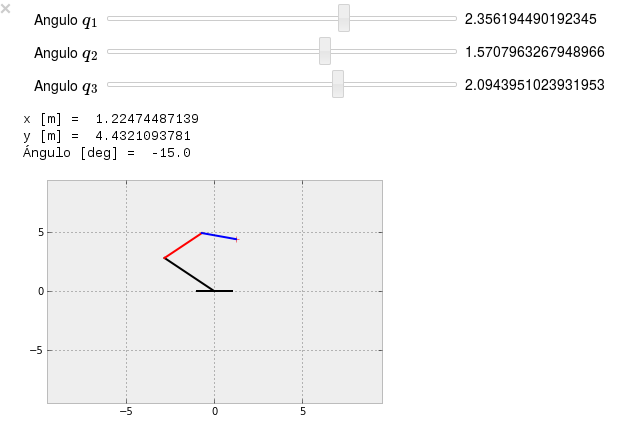
\includegraphics[width=500pt,keepaspectratio=True]{./cap_cin_dir.png}
 % P&ID_anti-suge.png: 0x0 pixel, 300dpi, 0.00x0.00 cm, bb=
  \textit{Figura 3: Captura de la ejecución del código en un Notebook de IPython}
\end{center}



\begin{multicols}{2}

\subsection{Cinemática Inversa}
Realizaremos la cinemática inversa mediate métodos geométricos. Sea Pher el punto desado de la herramienta con coordenadas
$x_h$ y $y_h$ ($z_h=0$ al tratarse de un robot plano) y formando un ángulo $\theta_h$ con la horizontal. \\
Por trigonometría las coordenadas de la articulación 3 serán
\(x_3 = x_h - l_3 * cos(\theta)\) y \(y_3 = y_h - l_3 * sin(\theta)\).
Podemos obtener \(q_1\) y \(q_2\) con
\(q_2 = arctg({{\pm \sqrt{1-cos^2 (q_2)}} \over {cos (q_2)}})\) donde
\(cos (q_2) = {{x_3^2 + y_3^2 - l_1^2 - l_2^2} \over {2 l_1 l_2}}\) y
\(q_1 = arctg({{y_3}\over{\pm x_3}})-arctg({{l_2 sin(q_2)} \over {l_1 + l_2 cos(q_2)}})\)
(Barrientos, Fundamentos de Robótica, 2007).

\end{multicols}
\subsubsection{Código en python}

\begin{Verbatim}[commandchars=\\\{\}]
{\color{incolor}In [{\color{incolor}2}]:} \PY{k+kn}{from} \PY{n+nn}{numpy} \PY{k+kn}{import} \PY{n}{sqrt}\PY{p}{,} \PY{n}{arcsin}
         \PY{k}{def} \PY{n+nf}{cin\PYZus{}inv}\PY{p}{(}\PY{n}{x}\PY{p}{,}\PY{n}{y}\PY{p}{,}\PY{n}{theta}\PY{p}{)}\PY{p}{:}
             \PY{n}{theta} \PY{o}{=} \PY{n}{theta} \PY{o}{/} \PY{n}{fact}
             \PY{n}{x\PYZus{}3} \PY{o}{=} \PY{n}{x} \PY{o}{\PYZhy{}} \PY{n}{l\PYZus{}3} \PY{o}{*} \PY{n}{cos}\PY{p}{(}\PY{n}{theta}\PY{p}{)}
             \PY{n}{y\PYZus{}3} \PY{o}{=} \PY{n}{y} \PY{o}{\PYZhy{}} \PY{n}{l\PYZus{}3} \PY{o}{*} \PY{n}{sin}\PY{p}{(}\PY{n}{theta}\PY{p}{)}
             \PY{n}{cos\PYZus{}q\PYZus{}2} \PY{o}{=} \PY{p}{(}\PY{n}{x\PYZus{}3}\PY{o}{*}\PY{o}{*}\PY{l+m+mi}{2} \PY{o}{+} \PY{n}{y\PYZus{}3}\PY{o}{*}\PY{o}{*}\PY{l+m+mi}{2} \PY{o}{\PYZhy{}} \PY{n}{l\PYZus{}1}\PY{o}{*}\PY{o}{*}\PY{l+m+mi}{2} \PY{o}{\PYZhy{}} \PY{n}{l\PYZus{}2}\PY{o}{*}\PY{o}{*}\PY{l+m+mi}{2}\PY{p}{)} \PY{o}{/} \PY{p}{(}\PY{l+m+mi}{2} \PY{o}{*} \PY{n}{l\PYZus{}1} \PY{o}{*} \PY{n}{l\PYZus{}2}\PY{p}{)}
             \PY{n}{q\PYZus{}2} \PY{o}{=} \PY{n}{arctan2}\PY{p}{(}\PY{n}{sqrt}\PY{p}{(}\PY{l+m+mi}{1} \PY{o}{\PYZhy{}} \PY{p}{(}\PY{n}{cos\PYZus{}q\PYZus{}2}\PY{p}{)}\PY{o}{*}\PY{o}{*}\PY{l+m+mi}{2}\PY{p}{)}\PY{p}{,}\PY{n}{cos\PYZus{}q\PYZus{}2}\PY{p}{)}
             \PY{n}{q\PYZus{}1} \PY{o}{=} \PY{n}{arctan2}\PY{p}{(}\PY{n}{y\PYZus{}3}\PY{p}{,}\PY{n}{x\PYZus{}3}\PY{p}{)} \PY{o}{\PYZhy{}} \PY{n}{arctan2}\PY{p}{(}\PY{p}{(}\PY{n}{l\PYZus{}2} \PY{o}{*} \PY{n}{sin}\PY{p}{(}\PY{n}{q\PYZus{}2}\PY{p}{)}\PY{p}{)}\PY{p}{,}\PY{p}{(}\PY{n}{l\PYZus{}1} \PY{o}{+} \PY{n}{l\PYZus{}2} \PY{o}{*} \PY{n}{cos\PYZus{}q\PYZus{}2}\PY{p}{)}\PY{p}{)}
             \PY{n}{l} \PY{o}{=} \PY{n}{sqrt}\PY{p}{(}\PY{n}{l\PYZus{}1}\PY{o}{*}\PY{o}{*}\PY{l+m+mi}{2} \PY{o}{+} \PY{n}{l\PYZus{}2}\PY{o}{*}\PY{o}{*}\PY{l+m+mi}{2} \PY{o}{\PYZhy{}} \PY{l+m+mi}{2} \PY{o}{*} \PY{n}{l\PYZus{}1} \PY{o}{*} \PY{n}{l\PYZus{}2} \PY{o}{*} \PY{n}{cos\PYZus{}q\PYZus{}2}\PY{p}{)}
             \PY{n}{alpha} \PY{o}{=} \PY{n}{arcsin}\PY{p}{(}\PY{n}{l\PYZus{}1} \PY{o}{*} \PY{n}{sin}\PY{p}{(}\PY{n}{q\PYZus{}2}\PY{p}{)} \PY{o}{/} \PY{n}{l}\PY{p}{)}
             \PY{n}{beta} \PY{o}{=} \PY{n}{arctan2}\PY{p}{(}\PY{n}{y\PYZus{}3}\PY{p}{,}\PY{n}{x\PYZus{}3}\PY{p}{)}
             \PY{n}{k} \PY{o}{=} \PY{n}{pi} \PY{o}{\PYZhy{}} \PY{n}{theta}
             \PY{n}{q\PYZus{}3} \PY{o}{=} \PY{p}{(}\PY{n}{alpha} \PY{o}{+} \PY{n}{k} \PY{o}{+} \PY{n}{beta}\PY{p}{)}
             \PY{n}{plt}\PY{o}{.}\PY{n}{plot}\PY{p}{(}\PY{n}{x}\PY{p}{,} \PY{n}{y}\PY{p}{,} \PY{l+s}{\PYZsq{}}\PY{l+s}{r+}\PY{l+s}{\PYZsq{}}\PY{p}{)}
             \PY{n}{plt}\PY{o}{.}\PY{n}{ylim}\PY{p}{(}\PY{o}{\PYZhy{}}\PY{l+m+mf}{9.5}\PY{p}{,} \PY{l+m+mf}{9.5}\PY{p}{)}
             \PY{n}{plt}\PY{o}{.}\PY{n}{xlim}\PY{p}{(}\PY{o}{\PYZhy{}}\PY{l+m+mf}{9.5}\PY{p}{,} \PY{l+m+mf}{9.5}\PY{p}{)}
             \PY{n}{plt}\PY{o}{.}\PY{n}{plot}\PY{p}{(}\PY{p}{[}\PY{o}{\PYZhy{}}\PY{l+m+mi}{1}\PY{p}{,}\PY{l+m+mi}{1}\PY{p}{]}\PY{p}{,}\PY{p}{[}\PY{l+m+mi}{0}\PY{p}{,}\PY{l+m+mi}{0}\PY{p}{]}\PY{p}{,}\PY{l+s}{\PYZsq{}}\PY{l+s}{k\PYZhy{}}\PY{l+s}{\PYZsq{}}\PY{p}{)}
             \PY{n}{x\PYZus{}2} \PY{o}{=} \PY{n}{l\PYZus{}1} \PY{o}{*} \PY{n}{cos}\PY{p}{(}\PY{n}{q\PYZus{}1}\PY{p}{)}
             \PY{n}{y\PYZus{}2} \PY{o}{=} \PY{n}{l\PYZus{}1} \PY{o}{*} \PY{n}{sin}\PY{p}{(}\PY{n}{q\PYZus{}1}\PY{p}{)}
             \PY{n}{x\PYZus{}1} \PY{o}{=} \PY{l+m+mi}{0}
             \PY{n}{y\PYZus{}1} \PY{o}{=} \PY{l+m+mi}{0}
             \PY{n}{plt}\PY{o}{.}\PY{n}{plot}\PY{p}{(}\PY{p}{[}\PY{n}{x\PYZus{}1}\PY{p}{,}\PY{n}{x\PYZus{}2}\PY{p}{]}\PY{p}{,}\PY{p}{[}\PY{n}{y\PYZus{}1}\PY{p}{,}\PY{n}{y\PYZus{}2}\PY{p}{]}\PY{p}{,}\PY{l+s}{\PYZsq{}}\PY{l+s}{r\PYZhy{}}\PY{l+s}{\PYZsq{}}\PY{p}{)}
             \PY{n}{plt}\PY{o}{.}\PY{n}{plot}\PY{p}{(}\PY{p}{[}\PY{n}{x\PYZus{}2}\PY{p}{,}\PY{n}{x\PYZus{}3}\PY{p}{]}\PY{p}{,}\PY{p}{[}\PY{n}{y\PYZus{}2}\PY{p}{,}\PY{n}{y\PYZus{}3}\PY{p}{]}\PY{p}{,}\PY{l+s}{\PYZsq{}}\PY{l+s}{b\PYZhy{}}\PY{l+s}{\PYZsq{}}\PY{p}{)}
             \PY{n}{plt}\PY{o}{.}\PY{n}{plot}\PY{p}{(}\PY{p}{[}\PY{n}{x\PYZus{}3}\PY{p}{,}\PY{n}{x}\PY{p}{]}\PY{p}{,}\PY{p}{[}\PY{n}{y\PYZus{}3}\PY{p}{,}\PY{n}{y}\PY{p}{]}\PY{p}{,}\PY{l+s}{\PYZsq{}}\PY{l+s}{k\PYZhy{}}\PY{l+s}{\PYZsq{}}\PY{p}{)}
             \PY{n}{plt}\PY{o}{.}\PY{n}{grid}\PY{p}{(}\PY{n+nb+bp}{True}\PY{p}{)}
             \PY{k}{print} \PY{l+s}{\PYZdq{}}\PY{l+s}{q1 [deg] = }\PY{l+s}{\PYZdq{}}\PY{p}{,} \PY{n}{q\PYZus{}1} \PY{o}{*} \PY{n}{fact}
             \PY{k}{print} \PY{l+s}{\PYZdq{}}\PY{l+s}{q2 [deg] = }\PY{l+s}{\PYZdq{}}\PY{p}{,} \PY{n}{q\PYZus{}2} \PY{o}{*} \PY{n}{fact}
             \PY{k}{print} \PY{l+s}{\PYZdq{}}\PY{l+s}{q3 [deg] = }\PY{l+s}{\PYZdq{}}\PY{p}{,} \PY{n}{q\PYZus{}3} \PY{o}{*} \PY{n}{fact}
             \PY{k}{print} \PY{l+s}{\PYZdq{}}\PY{l+s}{l1 [m] = }\PY{l+s}{\PYZdq{}}\PY{p}{,} \PY{n}{sqrt}\PY{p}{(}\PY{p}{(}\PY{n}{x\PYZus{}2}\PY{o}{*}\PY{o}{*}\PY{l+m+mi}{2}\PY{p}{)}\PY{o}{+}\PY{p}{(}\PY{n}{y\PYZus{}2}\PY{o}{*}\PY{o}{*}\PY{l+m+mi}{2}\PY{p}{)}\PY{p}{)}\PY{p}{,} \PY{n}{l\PYZus{}1}
             \PY{k}{print} \PY{l+s}{\PYZdq{}}\PY{l+s}{l2 [m] = }\PY{l+s}{\PYZdq{}}\PY{p}{,} \PY{n}{sqrt}\PY{p}{(}\PY{p}{(}\PY{p}{(}\PY{n}{x\PYZus{}2}\PY{o}{\PYZhy{}}\PY{n}{x\PYZus{}3}\PY{p}{)}\PY{o}{*}\PY{o}{*}\PY{l+m+mi}{2}\PY{p}{)}\PY{o}{+}\PY{p}{(}\PY{p}{(}\PY{n}{y\PYZus{}2}\PY{o}{\PYZhy{}}\PY{n}{y\PYZus{}3}\PY{p}{)}\PY{o}{*}\PY{o}{*}\PY{l+m+mi}{2}\PY{p}{)}\PY{p}{)}\PY{p}{,} \PY{n}{l\PYZus{}2}
             \PY{k}{print} \PY{l+s}{\PYZdq{}}\PY{l+s}{l3 [m] = }\PY{l+s}{\PYZdq{}}\PY{p}{,} \PY{n}{sqrt}\PY{p}{(}\PY{p}{(}\PY{p}{(}\PY{n}{x\PYZus{}3}\PY{o}{\PYZhy{}}\PY{n}{x}\PY{p}{)}\PY{o}{*}\PY{o}{*}\PY{l+m+mi}{2}\PY{p}{)}\PY{o}{+}\PY{p}{(}\PY{p}{(}\PY{n}{y\PYZus{}3}\PY{o}{\PYZhy{}}\PY{n}{y}\PY{p}{)}\PY{o}{*}\PY{o}{*}\PY{l+m+mi}{2}\PY{p}{)}\PY{p}{)}\PY{p}{,} \PY{n}{l\PYZus{}3}
         \PY{n}{x\PYZus{}slider} \PY{o}{=} \PY{n}{FloatSlider}\PY{p}{(}\PY{n+nb}{min}\PY{o}{=}\PY{o}{\PYZhy{}}\PY{l+m+mi}{9}\PY{p}{,} \PY{n+nb}{max}\PY{o}{=}\PY{l+m+mi}{9}\PY{p}{,} \PY{n}{step}\PY{o}{=}\PY{l+m+mf}{0.1}\PY{p}{,} \PY{n}{value}\PY{o}{=}\PY{o}{\PYZhy{}}\PY{l+m+mi}{1}\PY{p}{,} \PY{n}{description}\PY{o}{=}\PY{l+s}{\PYZsq{}}\PY{l+s}{X}\PY{l+s}{\PYZsq{}}\PY{p}{)}
         \PY{n}{y\PYZus{}slider} \PY{o}{=} \PY{n}{FloatSlider}\PY{p}{(}\PY{n+nb}{min}\PY{o}{=}\PY{o}{\PYZhy{}}\PY{l+m+mi}{9}\PY{p}{,} \PY{n+nb}{max}\PY{o}{=}\PY{l+m+mi}{9}\PY{p}{,} \PY{n}{step}\PY{o}{=}\PY{l+m+mf}{0.1}\PY{p}{,} \PY{n}{value}\PY{o}{=}\PY{l+m+mi}{4}\PY{p}{,} \PY{n}{description}\PY{o}{=}\PY{l+s}{\PYZsq{}}\PY{l+s}{Y}\PY{l+s}{\PYZsq{}}\PY{p}{)}
         \PY{n}{theta\PYZus{}slider} \PY{o}{=} \PY{n}{FloatSlider}\PY{p}{(}\PY{n+nb}{min}\PY{o}{=}\PY{l+m+mi}{0}\PY{p}{,} \PY{n+nb}{max}\PY{o}{=}\PY{l+m+mi}{360}\PY{p}{,} \PY{n}{step}\PY{o}{=}\PY{l+m+mf}{0.1}\PY{p}{,} \PY{n}{value}\PY{o}{=}\PY{l+m+mi}{200}\PY{p}{,} \PY{n}{description}\PY{o}{=}\PY{l+s}{\PYZsq{}}\PY{l+s}{Theta}\PY{l+s}{\PYZsq{}}\PY{p}{)}
         \PY{n}{w}\PY{o}{=}\PY{n}{interactive}\PY{p}{(}\PY{n}{cin\PYZus{}inv}\PY{p}{,}\PY{n}{x}\PY{o}{=}\PY{n}{x\PYZus{}slider}\PY{p}{,}\PY{n}{y}\PY{o}{=}\PY{n}{y\PYZus{}slider}\PY{p}{,}\PY{n}{theta}\PY{o}{=}\PY{n}{theta\PYZus{}slider}\PY{p}{)}
         \PY{n}{display}\PY{p}{(}\PY{n}{w}\PY{p}{)}
\end{Verbatim}

\begin{center}
 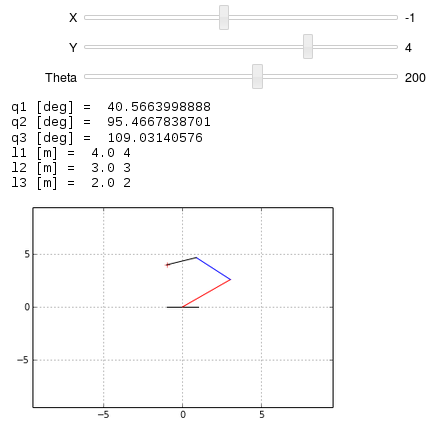
\includegraphics[width=480pt,keepaspectratio=True]{./cap_cin_inv.png}
  \textit{Figura 4: Captura de la ejecución del código en un Notebook de IPython}
\end{center}


\end{document}
